\documentclass[10pt,letterpaper]{report}
\usepackage[utf8]{inputenc}
\usepackage{amsmath}
\usepackage{amsfonts}
\usepackage{amssymb}
\usepackage{graphicx}
\author{Chun-Yi Wu}
\title{AST 381, HW 4}
\begin{document}

\maketitle


\begin{tabular}{|c|c|c|c|}
\hline 
• & $-\sigma$ & median & $+\sigma$ \\ 
\hline 
$t_0-2450000$ & 2853.06566990733 & 2853.07314048728 & 2853.08042829614 \\ 
\hline 
$P$ [day] & 3.52465765366727 & 3.52468468589338 & 3.52471150306524 \\ 
\hline 
$M_2\sin{i}$ [$M_{Jup}$] & 0.675930279625688 & 0.681384162438272 & 0.681651779379315 \\ 
\hline 
\end{tabular} 

\begin{figure} [h]
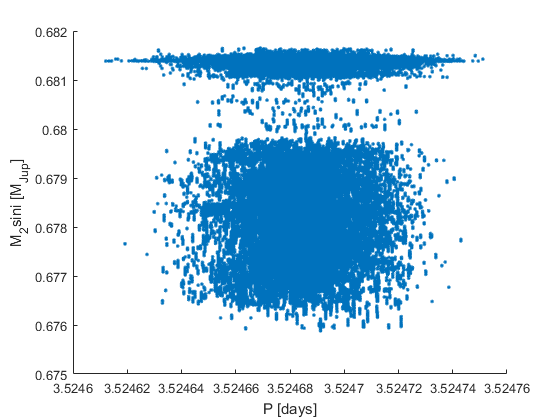
\includegraphics[scale=1]{scatter_PM.png}
\caption{Period vs. $M_2\sin{i}$}
\end{figure}

\begin{figure} [h]
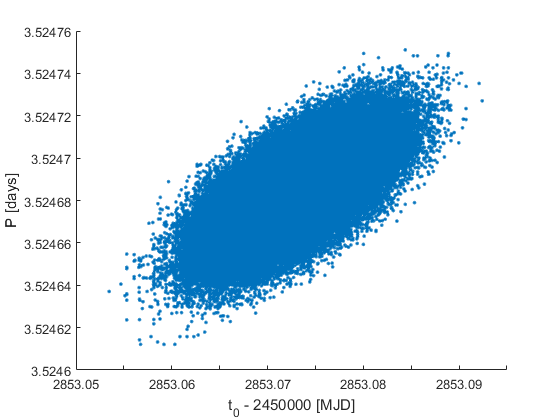
\includegraphics[scale=1]{scatter_t0P.png}
\caption{$t_0$ vs. Period}
\end{figure}

\begin{figure} [h]
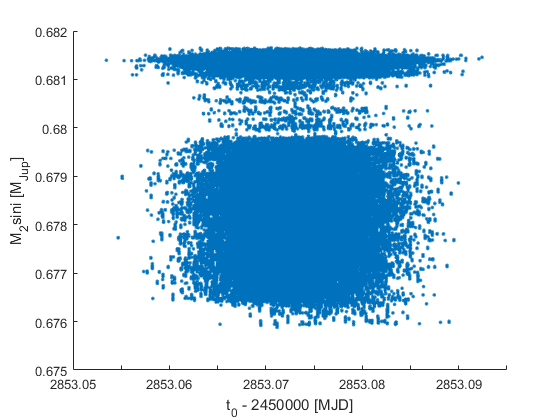
\includegraphics[scale=1]{scatter_t0M.png}
\caption{$t_0$ vs. $M_2\sin{i}$}
\end{figure}

\begin{figure} [h]
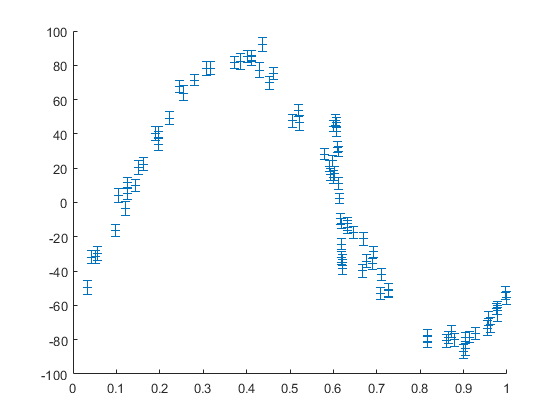
\includegraphics[scale=1]{periodgram.png}
\caption{phased RV curve}
\end{figure}

\newpage


\end{document}